\Chapter{Tesztek}
\label{Chap:tesztek}

%A játékmotor vizsgálata egy az egyben
%Review jellegű észrevételek
%Profilozás

Ez a fejezet az általam írt játékmotor, illetve az azzal megvalósított funkciók különböző megvalósításainak tesztjeiről szól. Különböző elemeket, különféle módszerrel lehet implementálni, többféleképp lehet optimalizálni, amelyek kirajzolási idejében különbségek vannak. Léteznek kisebb és nagyobb hatékonyságú algoritmusok a különböző problémák megoldására.

\section{Kirajzolási módszerek}

Alapvetően két fő kirajzolási módszer létezik az OpenGL-ben. Az egyik a régebbi glBegin-glEnd blokkos, a másik a modernebb Vertex Buffer Object-es (VBO). A kettő között a legfőbb különbség a gyorsaság. VBO-s megjelenítési mód esetén, mint ahogy a nevében is benne van, egy buffer-be (tárólóba) betöltjük az összes kirajzolni kívánt elemet, és azt egyben adjuk át a videokártyának, a legmegfelelőbb formátumban. Ez sokkal gyorsabb, mivel a régebbi egyesével adja át a pontokat kirajzolásra. \Aref{fig:old_fps}-es ábrán a régebbi, \aref{fig:vbo_fps}-es  ábrán pedig a VBO-s megjelenítési mód látható. Ugyanazoknak az objektumoknak a kirajzolása sokkal gyorsabb, ez látható mindkét képen a bal felső sarokban. Sokkal jobb a hardver kihasználtsága is, és az FPS (képkocka/másodperc) is kicsivel több, mint 8x magasabb.

\begin{figure}[h]
\centering
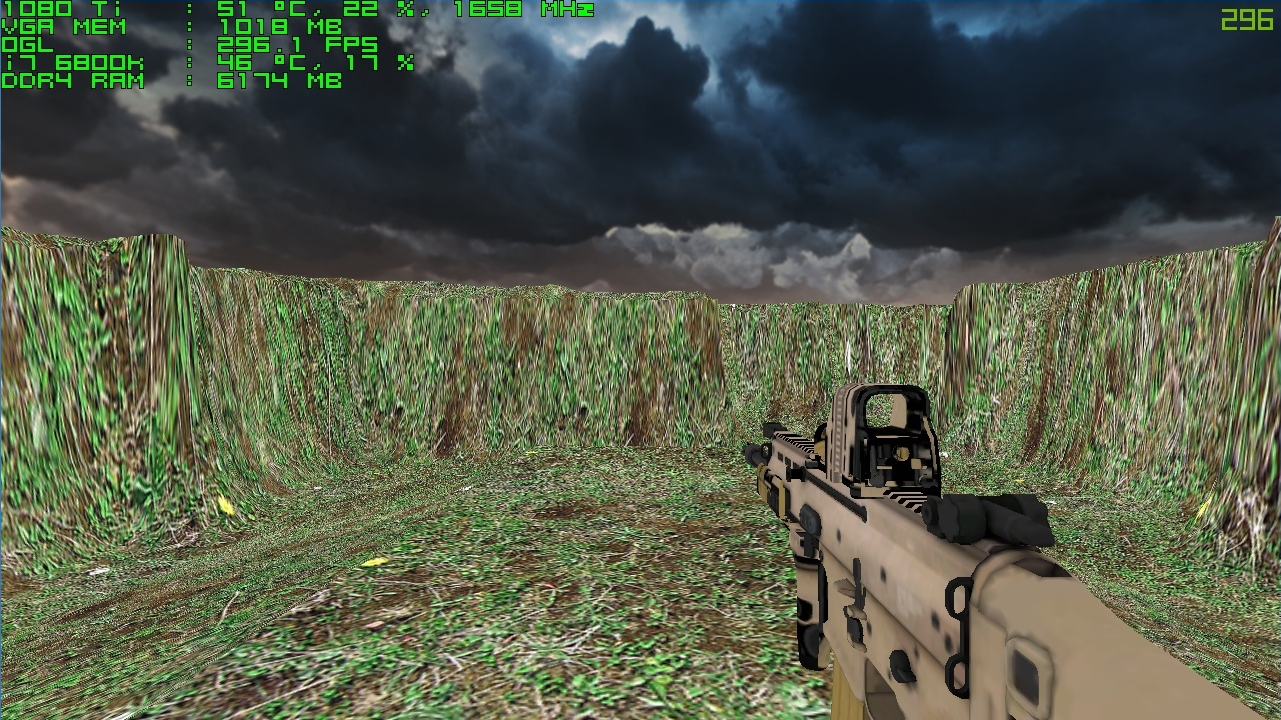
\includegraphics[scale=0.35]{kepek/old_method_fps.png}
\caption{A terep kirajzoltatása a régebbi módszerrel}
\label{fig:old_fps}
\end{figure}

\begin{figure}[h]
\centering
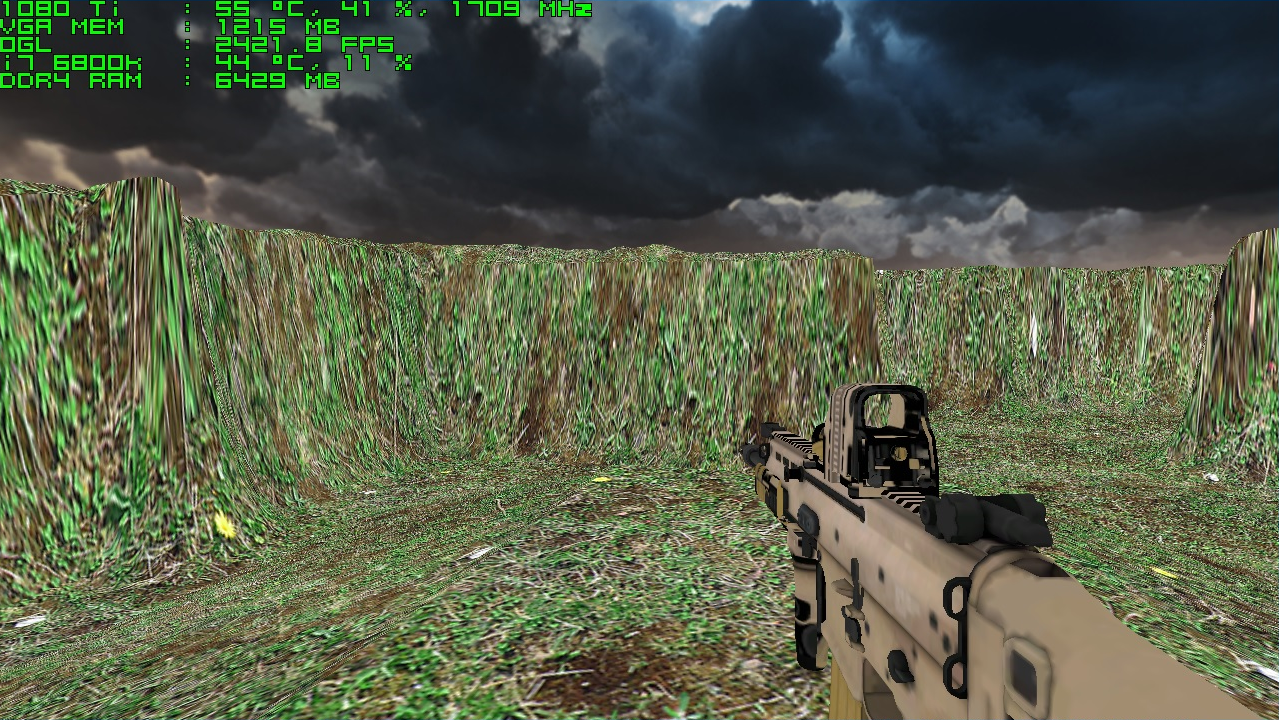
\includegraphics[scale=0.35]{kepek/vbo_method_fps.png}
\caption{A terep kirajzoltatása az újabb, VBO-s módszerrel}
\label{fig:vbo_fps}
\end{figure}

\section{Profilozás}

Ide még írni.
